\documentclass{article}
\usepackage[T1]{fontenc}
\usepackage[utf8]{inputenc}
\usepackage[polish]{babel}
\usepackage{amsmath}
\usepackage{url}
\usepackage{graphicx}
 \usepackage{float}
%{Informatyka stosowana 2022, I st., semestr VI}


\author{
	{Dominik Gałkowski, 247659} \\
	{Jan Śladowski, 247806}\\ 
{Prowadzący: dr inż. Marcin Kacprowicz}
}

\title{Komputerowe systemy rozpoznawania 2024/2025\\Projekt 2. Podsumowania lingwistyczne relacyjnych baz danych}
\begin{document}
\maketitle

Opis projektu ma formę artykułu naukowego lub raportu z zadania
badawczego (doświadczalnego/obliczeniowego (wg indywidualnych potrzeb związanych np. z
pracą inżynierską/naukową/zawodową). Wzory są numerowane, tablice są numerowane i podpisane nad
tablicą, rysunki są numerowane i podpisane pod rysunkiem. Podpis rysunku i
tabeli musi być wyczerpujący (nie ogólnikowy), aby czytelnik nie musiał sięgać do tekstu, aby go zrozumieć.\\
\indent {\bf Limit stron sprawozdania: 20. Nie zmieniać parametrów tekstu
(czcionki, marginesów, interlinii, itp.). Istotne dla sprawozdania rysunki,
tabele, informacje, kody itp. można umieścić w załącznikach, które nie wliczają
się do limitu stron.}\\
\indent {\bf Kolejne sekcje sprawozdania są uzupełniane wg wymagań w
opisie Projektu 2. i Harmonogramie Zajęć na WIKAMP KSR jako efekty zadań w~poszczególnych tygodniach}. 

\section{Cel}
Celem projektu jest stworzenie aplikacji, której główną funkcjonalnością
jest lingwistyczna agregacja zawartości wybranego zbioru danych. Ma ona za zadanie generowanie podsumowań lingwistycznych dla wybranych przez użytkownika kwantyfikatorów, sumaryzatorów i kwalifikatorów dla różnych atrybutów. Analiza otrzymanych wyników polega na określeniu, znaczenia wybranych kwantyfikatorów, sumaryzatorów, kwalifikatorów oraz miar ich jakości dla wiarygodności i jakości otrzymanych podsumowań lingwistycznych. Przykładowe podsumowanie to, np. większkość pomiarów ma wysoką wilgotność.

Zwięzły (2-3 zdania) opis
problemu, uwzględniający część eksperymentalną i
implementacyjną.  Opis (własny, nie skopiowany) zawiera przypisy do literatury (bibliografii) zamieszczonej na końcu sprawozdania
zgodnie z~Polską Normą (zob. materiały BG PŁ pt. ,,Bibliografia
załącznikowa'').\\ 
\indent Opis zawiera minimum teorii ściśle odniesionej do tego konkretnego zadania (zbiór
danych, liczba zmiennych i rekordów, jakie podsumowania chcesz generować i po
co, PRZYKŁADY, itp.), tak by inżynier innej specjalności zrozumiał dalszy
opis tego konkretnego eksperymentu. {\bf Nie przepisuj literatury -- pokaż na
przykładach jak
jej elementy wyglądają zastosowane konkretnie do Twojego zadania}. 
Nie przepisuj literatury ani teorii 
napisz krótko jak rozumiesz to co masz wykona¢: jakie działania, na
jakim zbiorze danych (link lub przypis), jaki jest spodziewany efekt.\\
\noindent {\bf Sekcja uzupełniona jako efekt zadania Tydzień 09 wg Harmonogramu Zajęć na WIKAMP KSR.}


\section{Baza danych, zmienne lingwistyczne, kwantyfikatory lingwistyczne}
\noindent {\bf Sekcja uzupełniona jako efekt zadania Tydzień 09 wg Harmonogramu Zajęć na WIKAMP KSR.}

\subsection{Charakterystyka podsumowywanej bazy danych}
W tym projekcie został wykorzystany zbiór danych zapisany w pliku w formacie .csv, na podstawie którego utworzono bazę danych - PostgresSQL. Baza danych o nazwie World Weather Repository zawiera różnego rodzaju pomiary danych atmosferycznych, np. temperatura lub prędkość wiatru. \cite{baza} Baza jest nabieżąco aktualizowana, natomiast na dzień 18.05.2025r. składa się z 71331 rekordów. 

Zmiennym lingwistycznym przypisuje się znaczenie ze względu na potrzebę lepszej interpretowalności danych przez użytkowników. Ludzie rzadko reagują na dokładne wartości (np. 1033.8 mb ciśnienia), natomiast określenie „wysokie ciśnienie” pozwala im intuicyjnie rozumieć sytuację pogodową. Stąd istnieje zapotrzebowanie na „przekładanie” danych formalnych na język naturalny. 
Podmiotem podsumowań jest pomiar, z bazy World Weather Repository wybrano 10 atrybutów, które zostaną rozmyte, są to następujące kolumny:
\begin{enumerate}
    \item last\_updated - data przeprowadzenia pomiarów, z tego atrybutu zostanie wykorzystana godzina w celu określenia pory dnia, zakres [0 - 24]. 
    \item temperature\_celsius - temperatura wyrażona w stopniach Celsjusza w zakresie [-25, 50].
    \item wind\_kph - prędkość wiatru wyrażona w kilometrach na godzinę w zakresie [3, 151]. 
    \item pressure\_mb - ciśnienie powietrza wyrażone w milibarach w zakresie [947 - 1050]. 
    \item humidity - wilgotność w zakresie [2 - 100\%].
    \item visibility\_km - widoczność wyrażona w kilometrach w zakresie [0, 32].
    \item uv\_index - wartość promieniowania słonecznego w zakresie [0, 16].
    \item air\_quality\_Carbon\_Monoxide - pomiar jakości powietrza ze względu na stężenie tlenku węgla w zakresie [0 - 2220].
    \item air\_quality\_Nitrogen\_dioxide - pomiar jakości powietrza ze względu na stężenie dwutlenku azotu w zakresie [0 - 428].
    \item air\_quality\_gb-defra-index - skala określająca poziomy zanieczyszczenia w powietrzu w zakresie [1 - 10].

    \begin{figure}[h!]
    \centering
    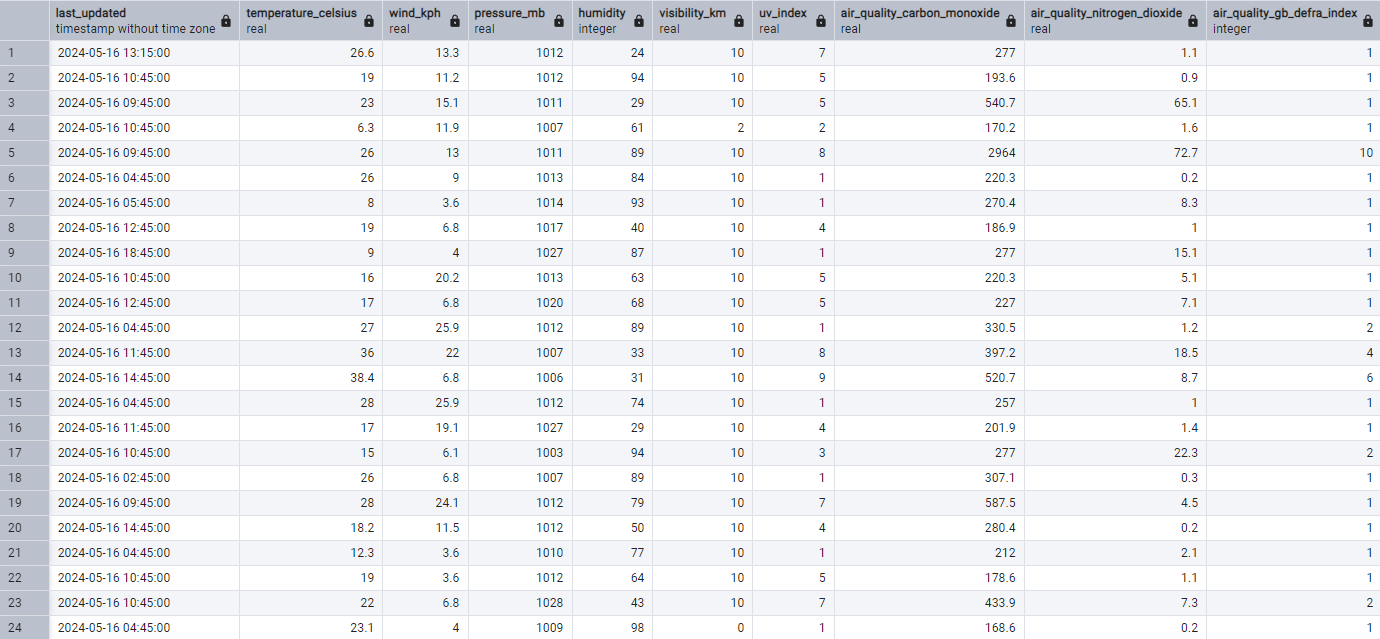
\includegraphics[width=\textwidth]{img/table.png}
    \caption{Fragment widoku tabeli z bazy danych.}
    \end{figure}
    
\end{enumerate}
Krótki opis bazy danych wybranej do podsumowywania, źródło, opis treści,
użyteczność/zastosowania. Liczba rekordów (min. $10\,000$ i koniecznie wszystkie tego
samego typu), liczba atrybutów możliwych do rozmycia (min. $10$), czyli o stosunkowo dużej
liczbie możliwych wartości. Zwyczajowe wartości lingwistyczne nadawane wybranym
atrybutom oraz dlaczego istnieje zwyczaj, zapotrzebowanie/inne powody
,,przekałdania'' tych danych na język
naturalny (a nie formalny) \cite{niewiadomski19, niewiadomski08}.\\
Realizacja bazy w wybranym DBMS. Rysunek lub tabela (fragment).

\subsection{Zmienne lingwistyczne (atrybuty/własności obiektów)}
Poniżej zostały zaprezentowane zmienne lingwistyczne dla atrybutów opisanych w sekcji 2.1, ich wzory analityczne oraz wykresy funkcji przynależności wraz z dopasowanymi do nich etykietami. W każdym z poniższych wzorów \(L_x\) to zmienna ligwistyczna, ..., \(H_x\) zbiór możliwych przyjmowanych wartości, \(X_x\) - przestrzeń rozważań, \(x\) - numer kolejnej zmiennej ligwistycznej. 
\begin{enumerate}
    \item last\_updated
        \begin{equation}
            L_1 = \langle \mathcal{L}_1, H_1, \mathcal{X}_1 \rangle
        \end{equation}
        gdzie: $\mathcal{L}_1$ – pora dnia, $H_1$ – \{noc, poranek, południe, popołudnie, wieczór\}, $\mathcal{X}_1 = [0, 24]$. \\
        Poniżej wzory dla wszystkich możliwych etykiet.
        \begin{equation}
            \mu_{\text{noc}}(x) =
            \begin{cases}
            \frac{8 - x}{3}, & x \in (5, 8] \\
            1, & x \in [0, 5] \\
            \frac{x - 21}{3}, & x \in [21, 24) \\
            0, & \text{w przeciwnym razie} \\
            \end{cases}
        \end{equation}

        \begin{equation}
            \mu_{\text{rano}}(x) =
            \begin{cases}
            \frac{x - 5}{2}, & x \in (5, 7] \\
            1, & x \in [7, 10] \\
            \frac{12 - x}{2}, & x \in (10, 12) \\
            0, & \text{w przeciwnym razie} \\
            \end{cases}
        \end{equation}

        \begin{equation}
            \mu_{\text{południe}}(x) =
            \begin{cases}
            \frac{x - 10}{1}, & x \in (10, 11] \\
            1, & x \in [11, 13] \\
            \frac{15 - x}{2}, & x \in (13, 15) \\
            0, & \text{w przeciwnym razie} \\
            \end{cases}
        \end{equation}

        \begin{equation}
            \mu_{\text{popołudnie}}(x) =
            \begin{cases}
            \frac{x - 15}{1}, & x \in (15, 16] \\
            1, & x \in [16, 18] \\
            \frac{20 - x}{2}, & x \in (18, 20) \\
            0, & \text{w przeciwnym razie} \\
             \end{cases}
        \end{equation}

        \begin{equation}
            \mu_{\text{wieczór}}(x) =
            \begin{cases}
            \frac{x - 19}{1}, & x \in (19, 20] \\
            1, & x \in [20, 22] \\
            \frac{24 - x}{2}, & x \in (22, 24) \\
            0, & \text{w przeciwnym razie} \\
            \end{cases}
        \end{equation} 
        
    \begin{figure}[H]
    \centering
    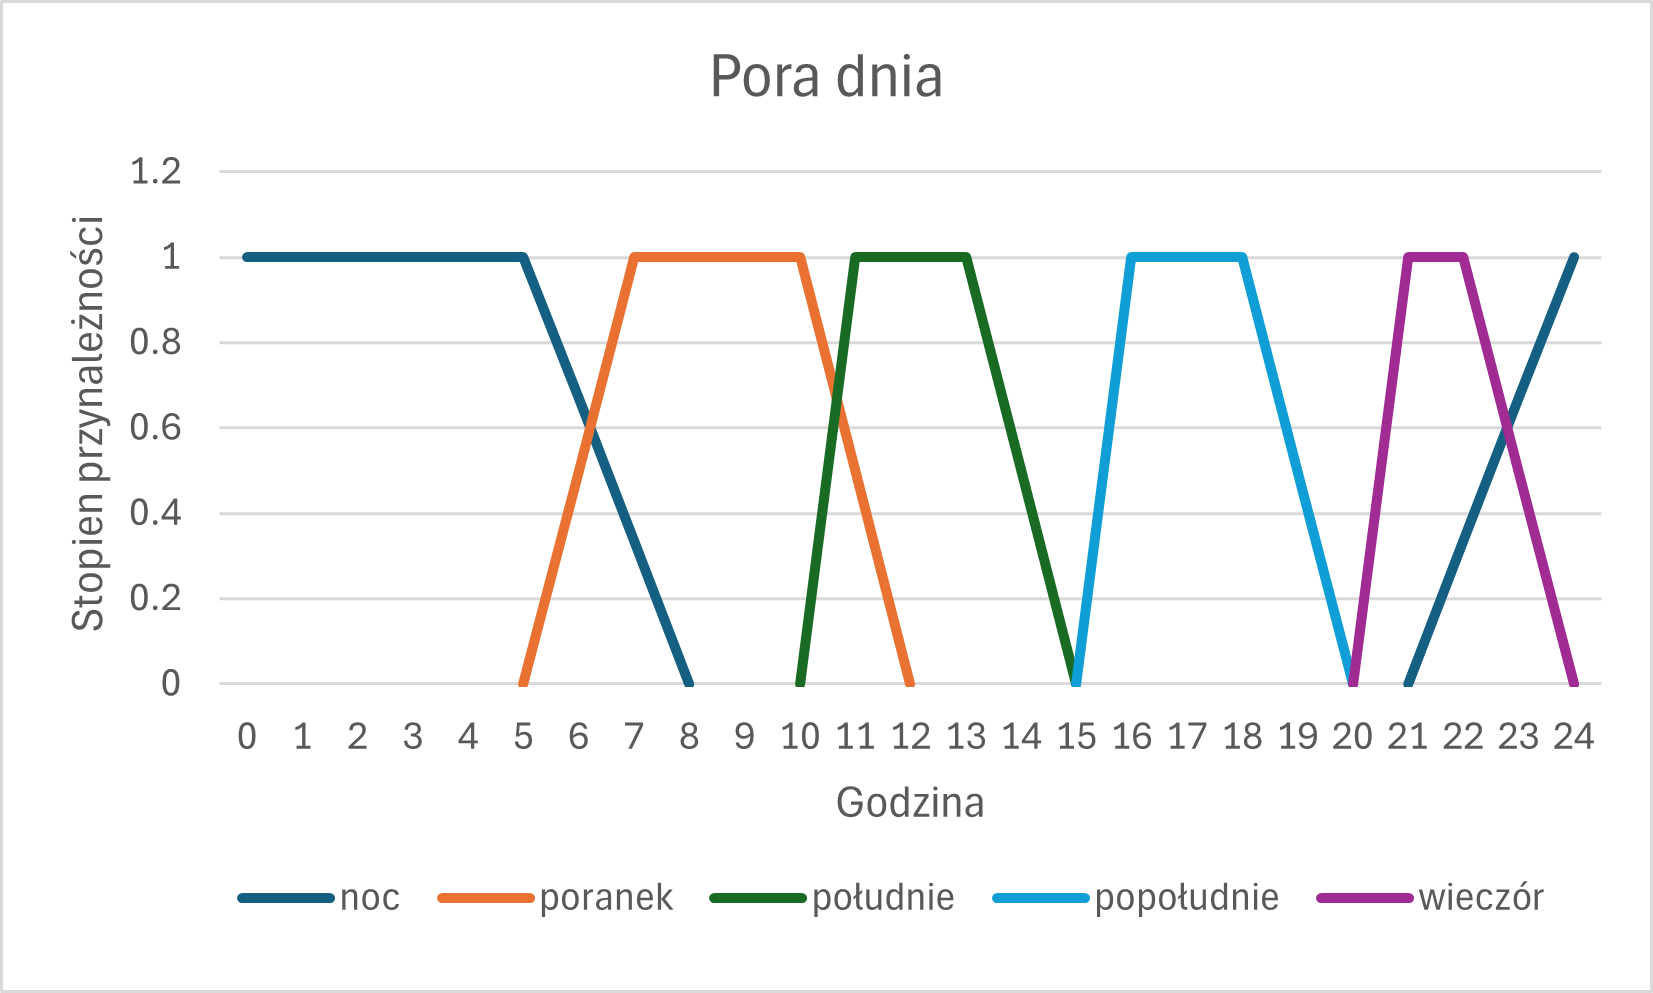
\includegraphics[width=\textwidth]{img/day.png}
    \caption{Wykres funkcji przynależności dla pory dnia.}
    \end{figure}
    
    \item temperature\_celsius
        \begin{equation}
            L_2 = \langle \mathcal{L}_2, H_2, \mathcal{X}_2 \rangle
        \end{equation}
        gdzie: $\mathcal{L}_2$ – temperatura, $H_2$ – \{bardzo zimno, zimno, umiarkowanie, ciepło, gorąco\}, $\mathcal{X}_2 = [-25, 50]$. \\
        Poniżej wzory dla wszystkich możliwych etykiet.
                \begin{equation}
                   \mu_{\text{bardzo\_zimno}}(x) =
                    \begin{cases}
                    1, & x \in [-25, -15] \\
                    \frac{-5 - x}{10}, & x \in (-15, -5] \\
                    0, & \text{w przeciwnym razie}
                    \end{cases}
                \end{equation}
                
                \begin{equation}
                   \mu_{\text{zimno}}(x) =
                    \begin{cases}
                    \frac{x + 10}{10}, & x \in (-10, 0] \\
                    1, & x \in (0, 5] \\
                    \frac{10 - x}{5}, & x \in (5, 10] \\
                    0, & \text{w przeciwnym razie}
                    \end{cases}
                \end{equation}

                \begin{equation}
                    \mu_{\text{umiarkowanie}}(x) =
                    \begin{cases}
                    \frac{x - 5}{5}, & x \in (5, 10] \\
                    1, & x \in (10, 15] \\
                    \frac{20 - x}{5}, & x \in (15, 20] \\
                    0, & \text{w przeciwnym razie}
                    \end{cases}
                \end{equation}

                \begin{equation}
                    \mu_{\text{ciepło}}(x) =
                    \begin{cases}
                    \frac{x - 15}{5}, & x \in (15, 20] \\
                    1, & x \in (20, 25] \\
                    \frac{30 - x}{5}, & x \in (25, 30] \\
                    0, & \text{w przeciwnym razie}
                    \end{cases}
                \end{equation}

                \begin{equation}
                    \mu_{\text{gorąco}}(x) =
                    \begin{cases}
                    \frac{x - 25}{10}, & x \in (25, 35] \\
                    1, & x \in (35, 50] \\
                    0, & \text{w przeciwnym razie}
                    \end{cases}
                \end{equation}

        \begin{figure}[H]
    \centering
    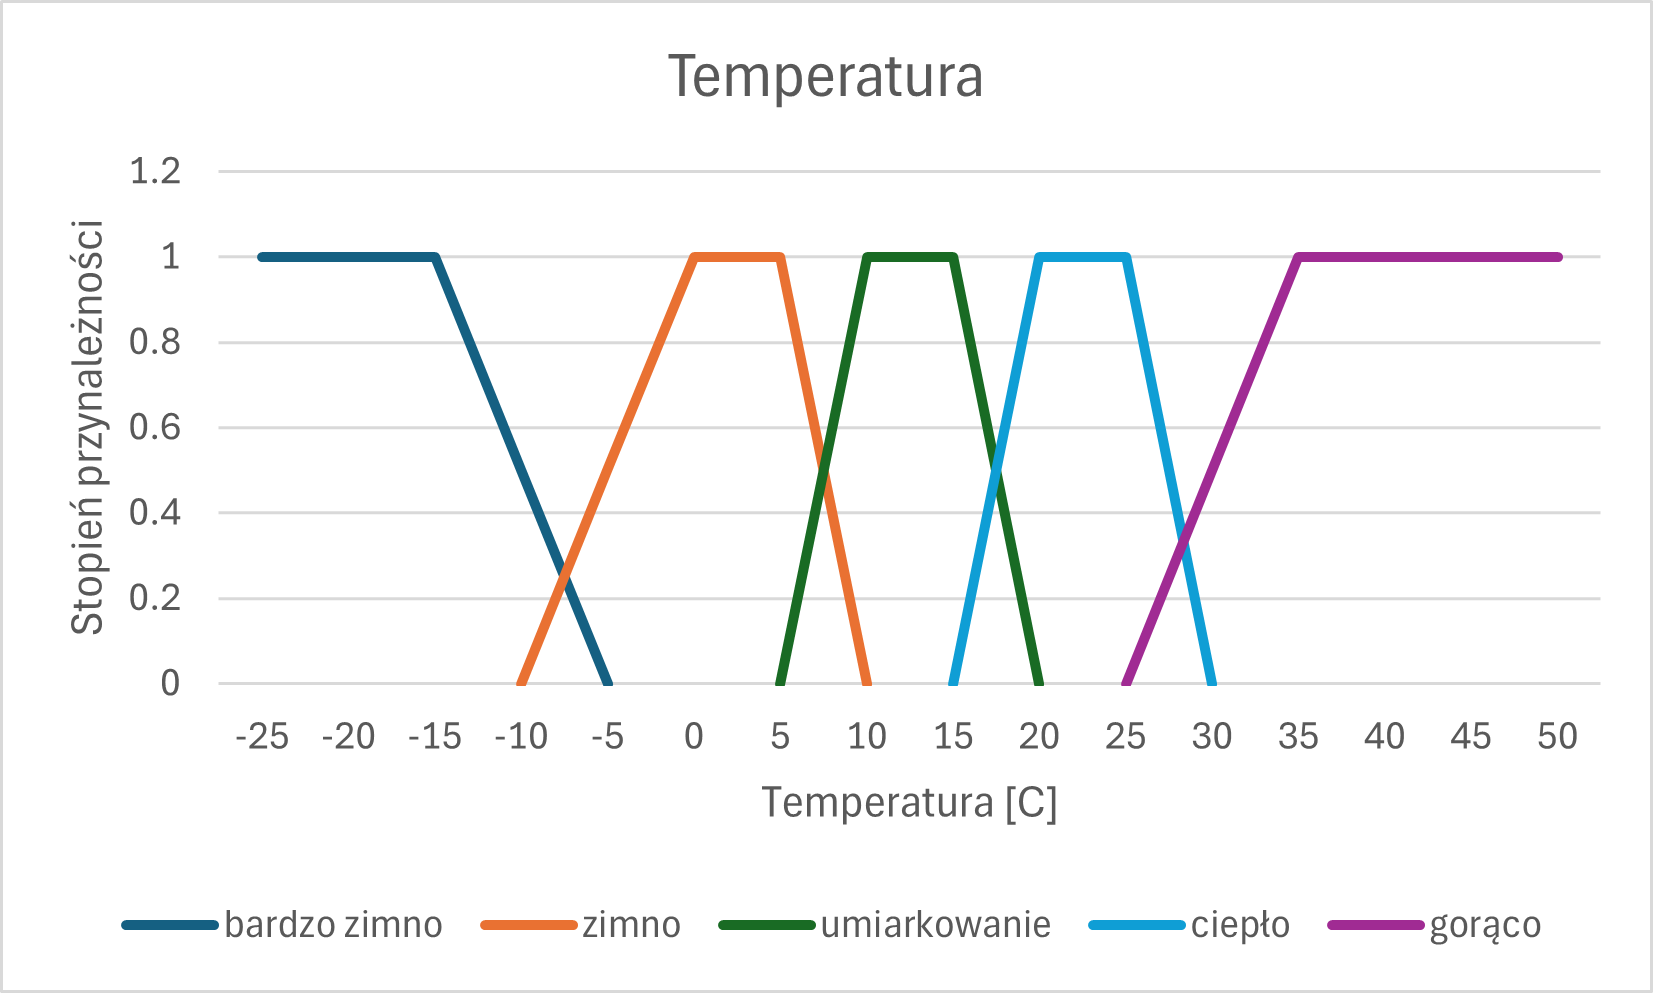
\includegraphics[width=\textwidth]{img/temp.png}
    \caption{Wykres funkcji przynależności dla temperatury.}
    \end{figure}

    \item wind\_kph
        \begin{equation}
            L_2 = \langle \mathcal{L}_2, H_2, \mathcal{X}_2 \rangle
        \end{equation}
        gdzie: $\mathcal{L}_3$ – siła wiatru, $H_3$ – \{słaby, umiarkowany, silny, bardzo silny\}, $\mathcal{X}_3 = [3, 151]$. \\
        Poniżej wzory dla wszystkich możliwych etykiet.
                  \begin{equation}
                    \mu_{\text{słaby}}(x) =
                    \begin{cases}
                    1, & x \in [3,  10] \\
                    \frac{20 - x}{10}, & x \in (10, 20] \\
                    0, & \text{w przeciwnym razie}
                    \end{cases}
                  \end{equation}
                \begin{equation}
                    \mu_{\text{umiarkowany}}(x) =
                    \begin{cases}
                    \frac{x - 10}{10}, & x \in (10, 20] \\
                    1, & x \in (20, 40] \\
                    \frac{60 - x}{20}, & x \in (40, 60] \\
                    0, & \text{w przeciwnym razie}
                    \end{cases}
                  \end{equation}
                \begin{equation}
                    \mu_{\text{silny}}(x) =
                    \begin{cases}
                    \frac{x - 40}{20}, & x \in (40, 60] \\
                    1, & x \in (60, 90] \\
                    \frac{110 - x}{20}, & x \in (90, 110] \\
                    0, & \text{w przeciwnym razie}
                    \end{cases}
              \end{equation}
                \begin{equation}
                    \mu_{\text{bardzo\_silny}}(x) =
                    \begin{cases}
                    \frac{x - 90}{20}, & x \in (90, 110] \\
                    1, & x \in (110, 152] \\
                    0, & \text{w przeciwnym razie}
                    \end{cases}
              \end{equation}

        \begin{figure}[H]
    \centering
    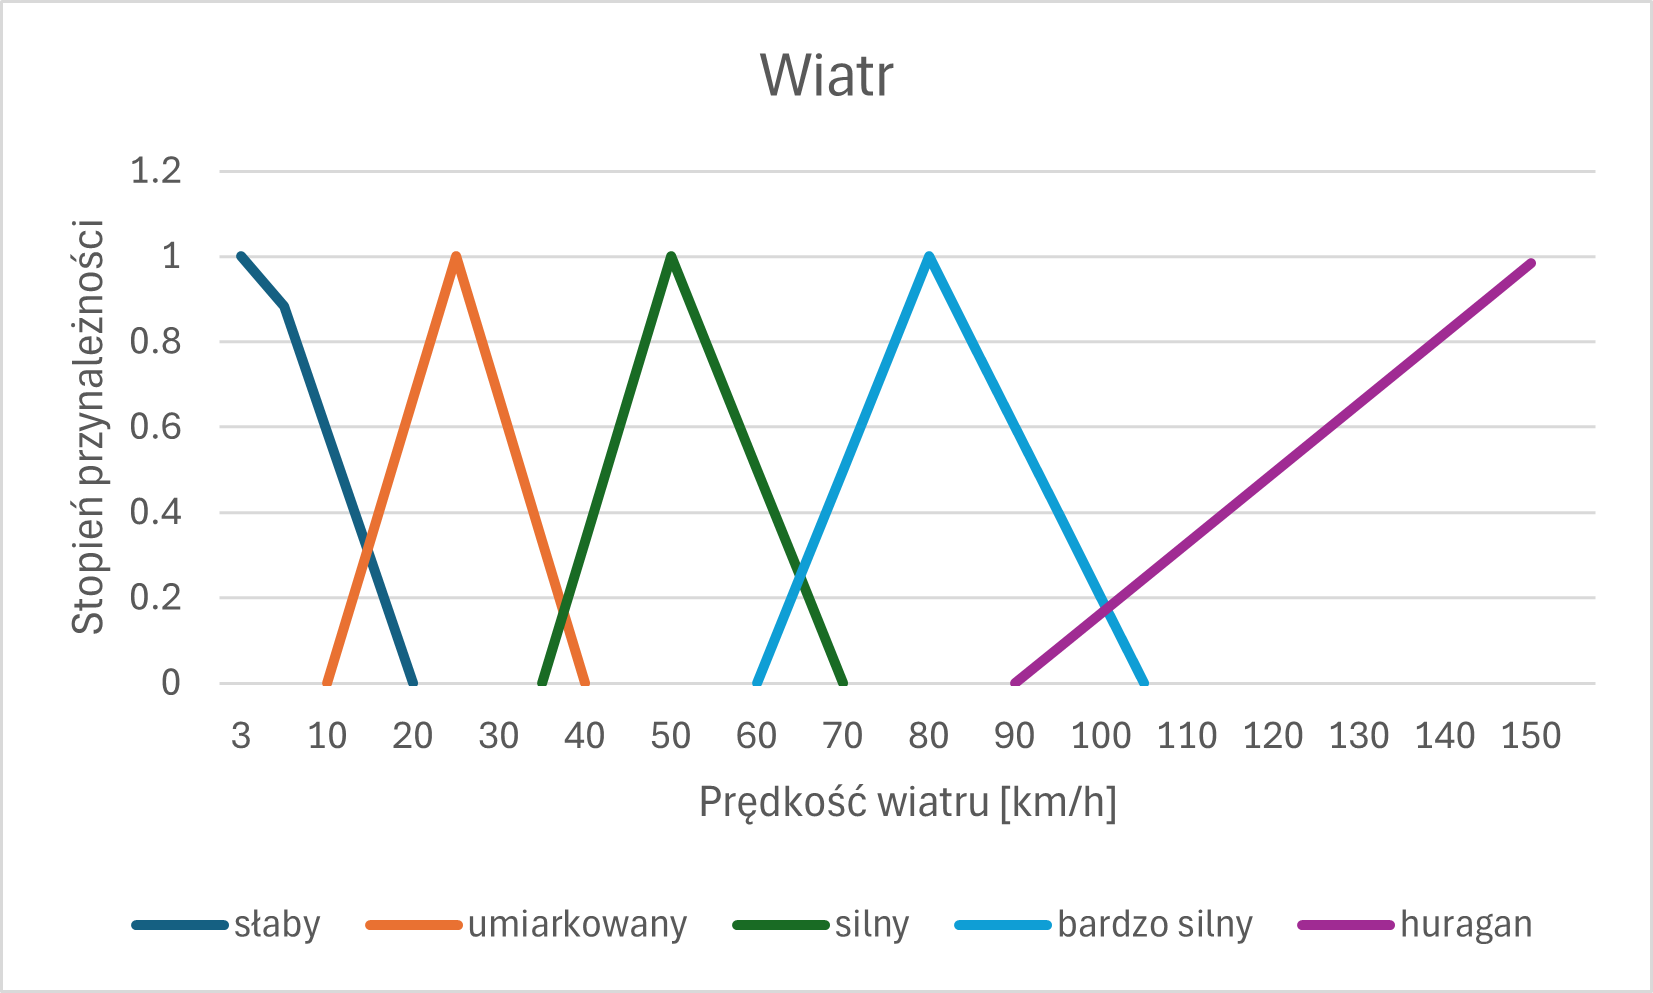
\includegraphics[width=\textwidth]{img/wind.png}
    \caption{Wykres funkcji przynależności dla siły wiatru.}
    \end{figure}
              
    \item pressure\_mb
        \begin{equation}
            L_4 = \langle \mathcal{L}_4, H_4, \mathcal{X}_4 \rangle
        \end{equation}
        gdzie: $\mathcal{L}_4$ – ciśnienie, $H_4$ – \{niskie, normalne, wysokie\}, $\mathcal{X}_4 = [947, 1050]$. \\
        Poniżej wzory dla wszystkich możliwych etykiet.
                \begin{equation}
                    \mu_{\text{niskie}}(x) =
                    \begin{cases}
                    1, & x \in [947, 970] \\
                    \frac{1000 - x}{30}, & x \in (970, 1000] \\
                    0, & \text{w przeciwnym razie}
                    \end{cases}
              \end{equation}
                \begin{equation}
                   \mu_{\text{normalne}}(x) =
                    \begin{cases}
                    \frac{x - 970}{30}, & x \in (970, 1000] \\
                    1, & x \in (1000, 1020] \\
                    \frac{1040 - x}{20}, & x \in (1020, 1040] \\
                    0, & \text{w przeciwnym razie}
                    \end{cases}
                \end{equation}

                \begin{equation}
                \mu_{\text{wysokie}}(x) =
                    \begin{cases}
                    \frac{x - 1020}{20}, & x \in (1020, 1040] \\
                    1, & x \in (1040, 1050] \\
                    0, & \text{w przeciwnym razie}
                    \end{cases}
                \end{equation}

    \begin{figure}[H]
    \centering
    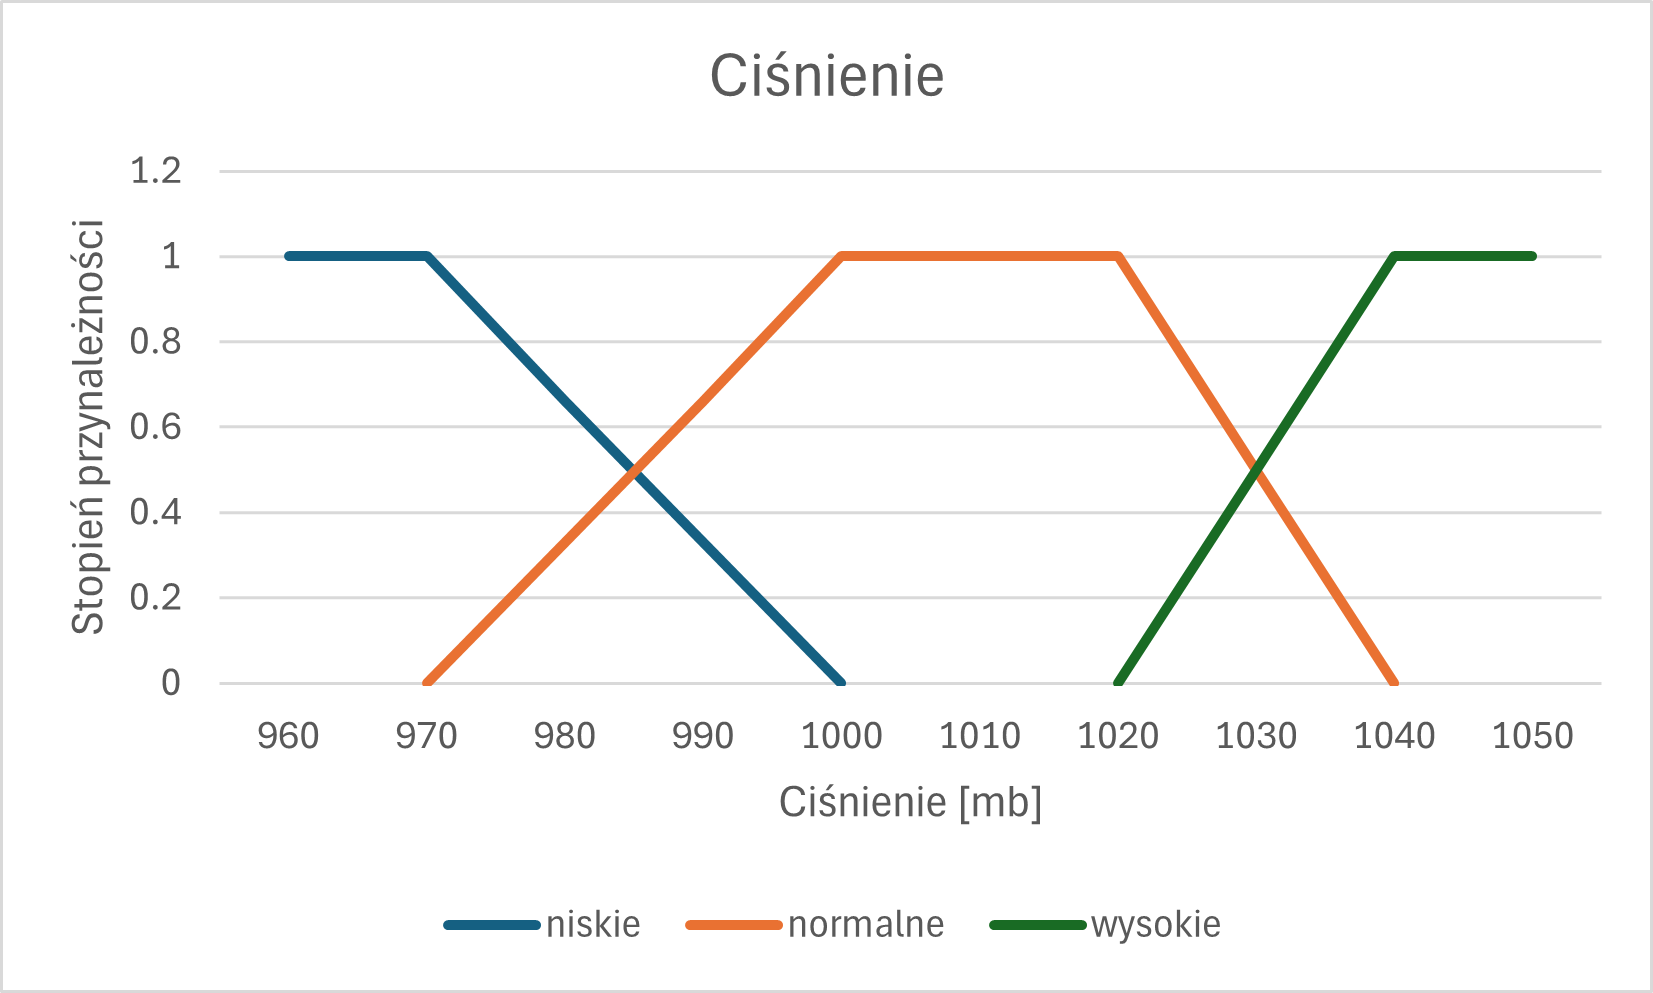
\includegraphics[width=\textwidth]{img/pressure.png}
    \caption{Wykres funkcji przynależności dla ciśnienia.}
    \end{figure}
    
    \item humidity
    \begin{equation}
            L_5 = \langle \mathcal{L}_5, H_5, \mathcal{X}_5 \rangle
        \end{equation}
        gdzie: $\mathcal{L}_5$ – stopień wilgotności, $H_5$ – \{sucho, umiarkowanie, wilgotno\}, $\mathcal{X}_1 = [2, 100]$. \\
        Poniżej wzory dla wszystkich możliwych etykiet.

\begin{equation}
\mu_{\text{sucho}}(x) =
\begin{cases}
1, & x \in [2, 30] \\
\frac{50 - x}{20}, & x \in (30, 50] \\
0, & \text{w przeciwnym razie}
\end{cases}
\end{equation}


\begin{equation}
\mu_{\text{umiarkowanie}}(x) =
\begin{cases}
\frac{x - 30}{20}, & x \in (30, 50] \\
1, & x \in (50, 70] \\
\frac{90 - x}{20}, & x \in (70, 90] \\
0, & \text{w przeciwnym razie}
\end{cases}
\end{equation}

\begin{equation}
\mu_{\text{wilgotno}}(x) =
\begin{cases}
\frac{x - 70}{20}, & x \in (70, 90] \\
1, & x \in (90, 100] \\
0, & \text{w przeciwnym razie}
\end{cases}
\end{equation}

    \begin{figure}[H]
    \centering
    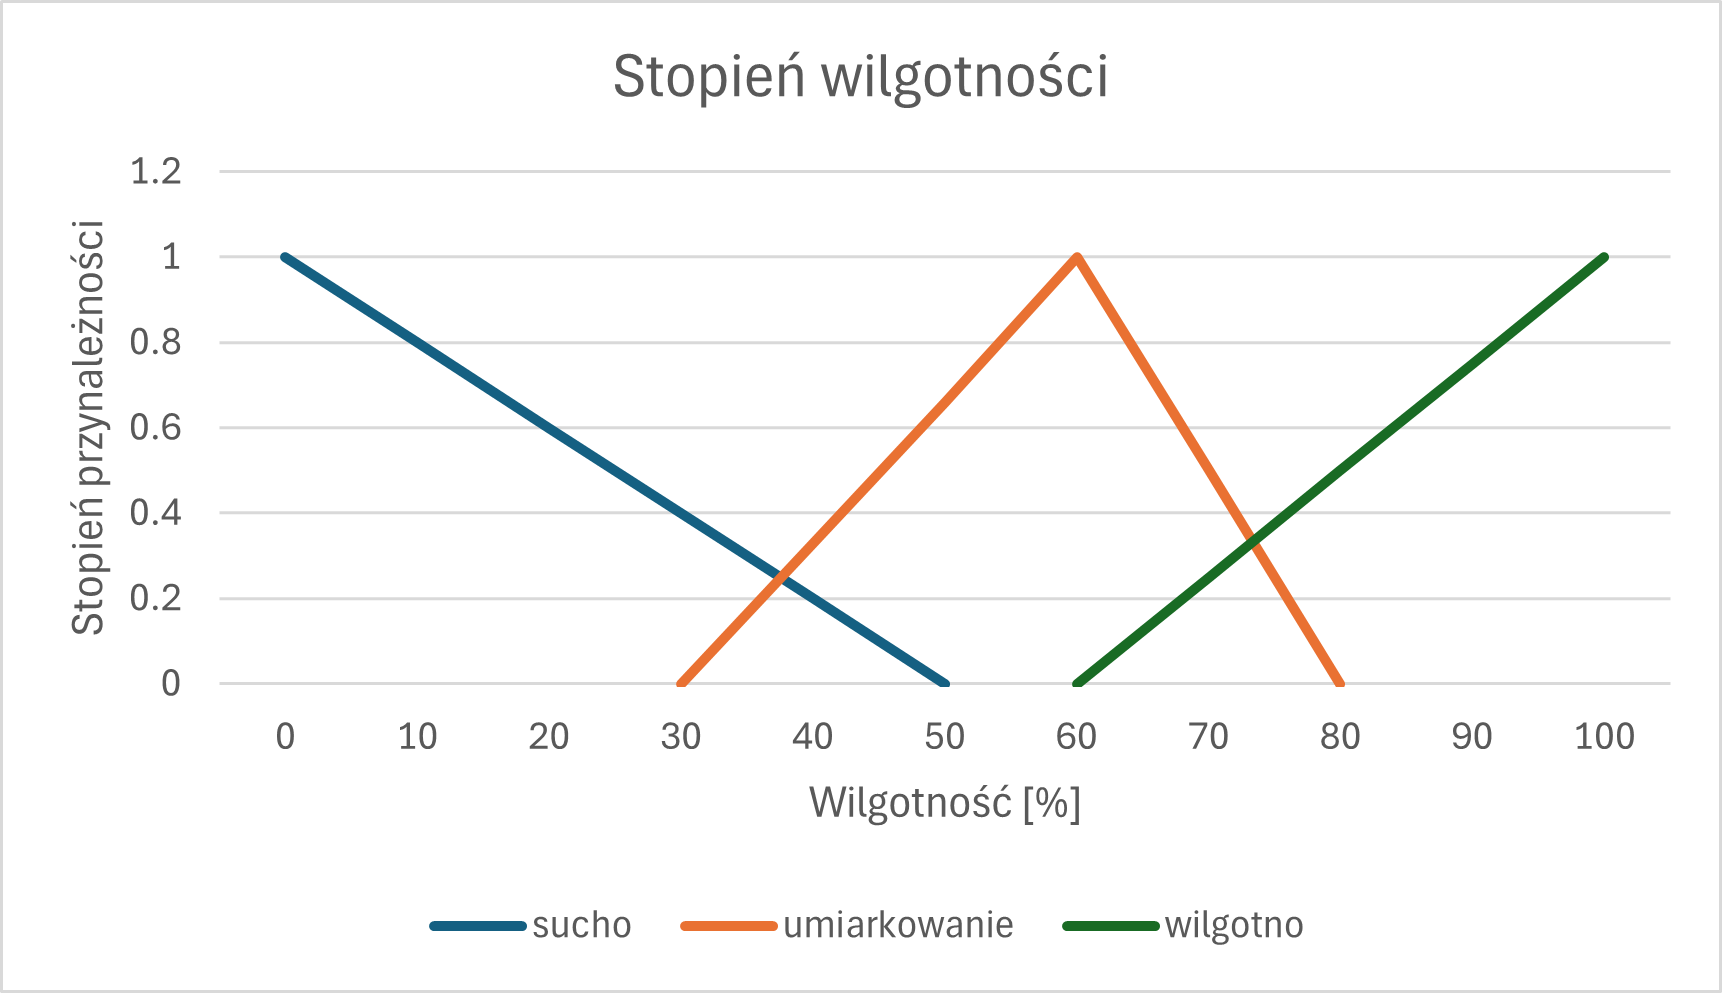
\includegraphics[width=\textwidth]{img/humidity.png}
    \caption{Wykres funkcji przynależności dla stopnia wilgotności.}
    \end{figure}

    \item visibility\_km
    \begin{equation}
            L_6 = \langle \mathcal{L}_6, H_6, \mathcal{X}_6 \rangle
        \end{equation}
        gdzie: $\mathcal{L}_6$ – stopień widoczności, $H_6$ – \{słaba, umiarkowana, dobra, bardzo dobra\}, $\mathcal{X}_6 = [0, 32]$. \\
        Poniżej wzory dla wszystkich możliwych etykiet.
\begin{equation}
\mu_{\text{słaba}}(x) =
\begin{cases}
1, & x \in [0, 4] \\
\frac{8 - x}{4}, & x \in (4, 8] \\
0, & \text{w przeciwnym razie}
\end{cases}
\end{equation}

\begin{equation}
\mu_{\text{umiarkowana}}(x) =
\begin{cases}
\frac{x - 4}{4}, & x \in (4, 8] \\
1, & x \in (8, 12] \\
\frac{16 - x}{4}, & x \in (12, 16] \\
0, & \text{w przeciwnym razie}
\end{cases}
\end{equation}

\begin{equation}
\mu_{\text{dobra}}(x) =
\begin{cases}
\frac{x - 12}{4}, & x \in (12, 16] \\
1, & x \in (16, 24] \\
\frac{28 - x}{4}, & x \in (24, 28] \\
0, & \text{w przeciwnym razie}
\end{cases}
\end{equation}

\begin{equation}
\mu_{\text{bardzo\_dobra}}(x) =
\begin{cases}
\frac{x - 24}{4}, & x \in (24, 28] \\
1, & x \in (28, 32] \\
0, & \text{w przeciwnym razie}
\end{cases}
\end{equation}

    \begin{figure}[H]
    \centering
    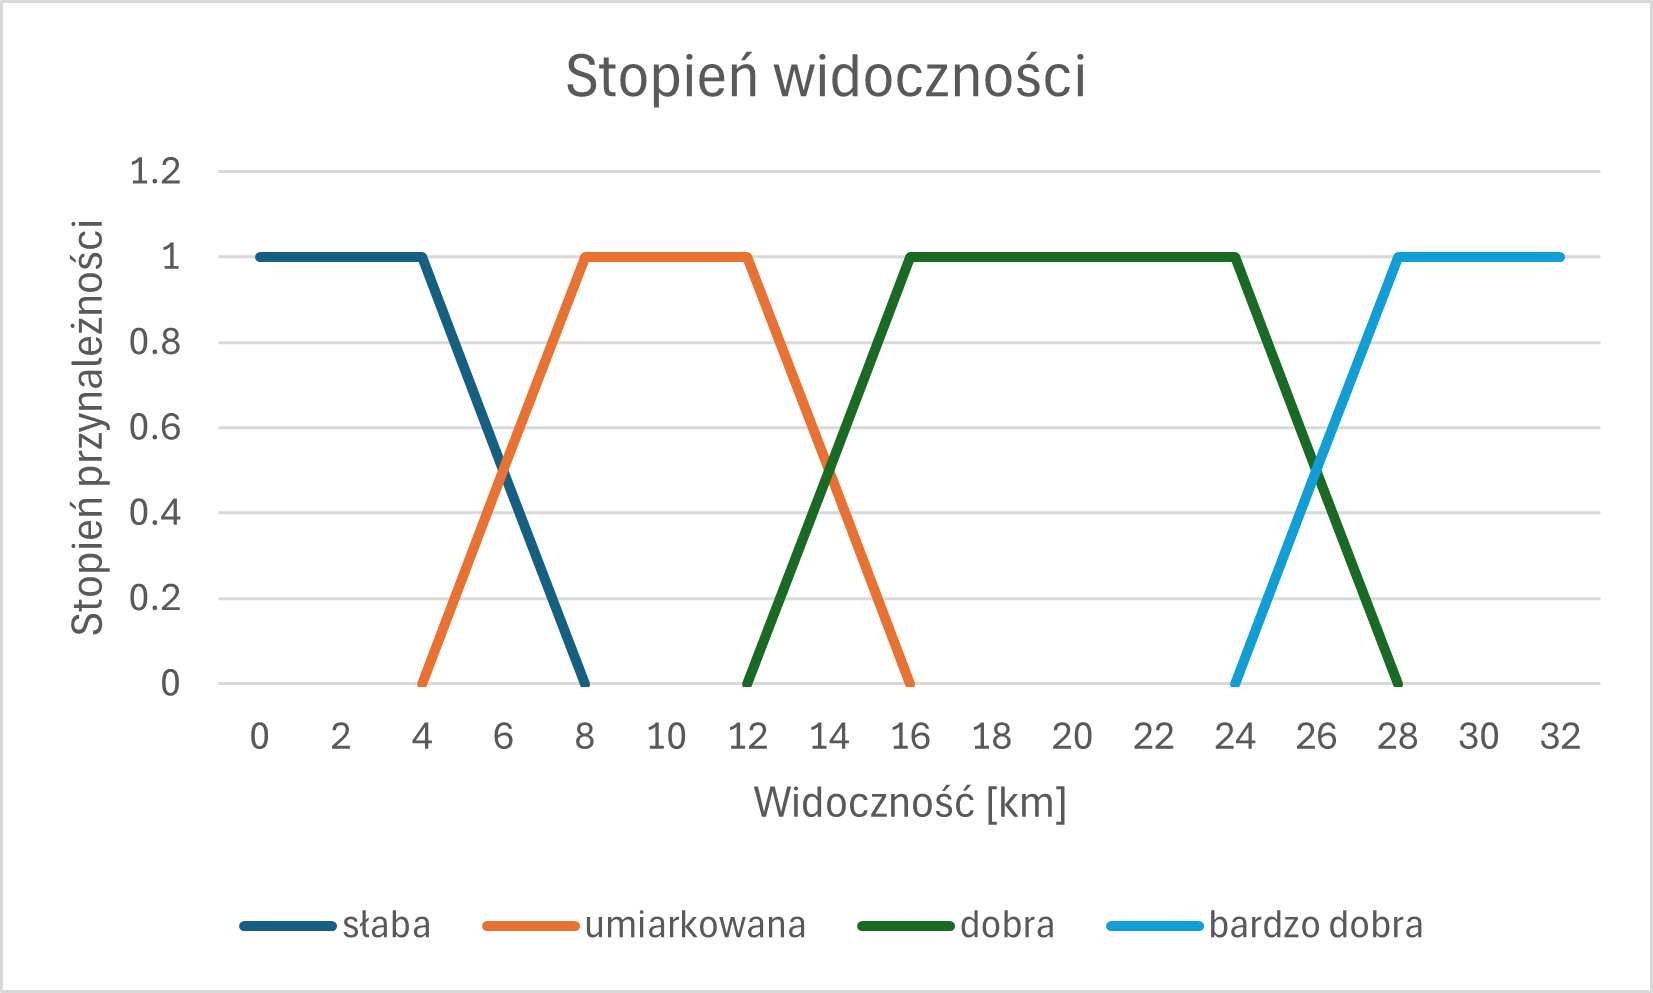
\includegraphics[width=\textwidth]{img/visibility.png}
    \caption{Wykres funkcji przynależności dla stopnia widoczności.}
    \end{figure}

    \item uv\_index
    \begin{equation}
            L_7 = \langle \mathcal{L}_7, H_7, \mathcal{X}_7 \rangle
        \end{equation}
        gdzie: $\mathcal{L}_7$ – promieniowanie UV, $H_1$ – \{niskie, umiarkowane, wysokie, bardzo wysokie, ekstremalne\}, $\mathcal{X}_7 = [0, 16]$. \\
        Poniżej wzory dla wszystkich możliwych etykiet.

\begin{equation}
\mu_{\text{niskie}}(x) =
\begin{cases}
1, & x \in [0, 2] \\
\frac{3 - x}{1}, & x \in (2, 3] \\
0, & \text{w przeciwnym razie}
\end{cases}
\end{equation}

\begin{equation}
\mu_{\text{umiarkowane}}(x) =
\begin{cases}
\frac{x - 2}{1}, & x \in (2, 3] \\
1, & x \in (3, 5] \\
\frac{6 - x}{1}, & x \in (5, 6) \\
0, & \text{w przeciwnym razie}
\end{cases}
\end{equation}

\begin{equation}
\mu_{\text{wysokie}}(x) =
\begin{cases}
\frac{x - 5}{1}, & x \in (5, 6] \\
1, & x \in (6, 7] \\
\frac{8 - x}{1}, & x \in (7, 8) \\
0, & \text{w przeciwnym razie}
\end{cases}
\end{equation}

\begin{equation}
\mu_{\text{bardzo\_wysokie}}(x) =
\begin{cases}
\frac{x - 7}{1}, & x \in (7, 8] \\
1, & x \in (8, 10] \\
\frac{11 - x}{1}, & x \in (10, 11) \\
0, & \text{w przeciwnym razie}
\end{cases}
\end{equation}

\begin{equation}
\mu_{\text{ekstremalne}}(x) =
\begin{cases}
\frac{x - 10}{1}, & x \in (10, 11] \\
1, & x \in (11, 16] \\
0, & \text{w przeciwnym razie}
\end{cases}
\end{equation}

    \begin{figure}[H]
    \centering
    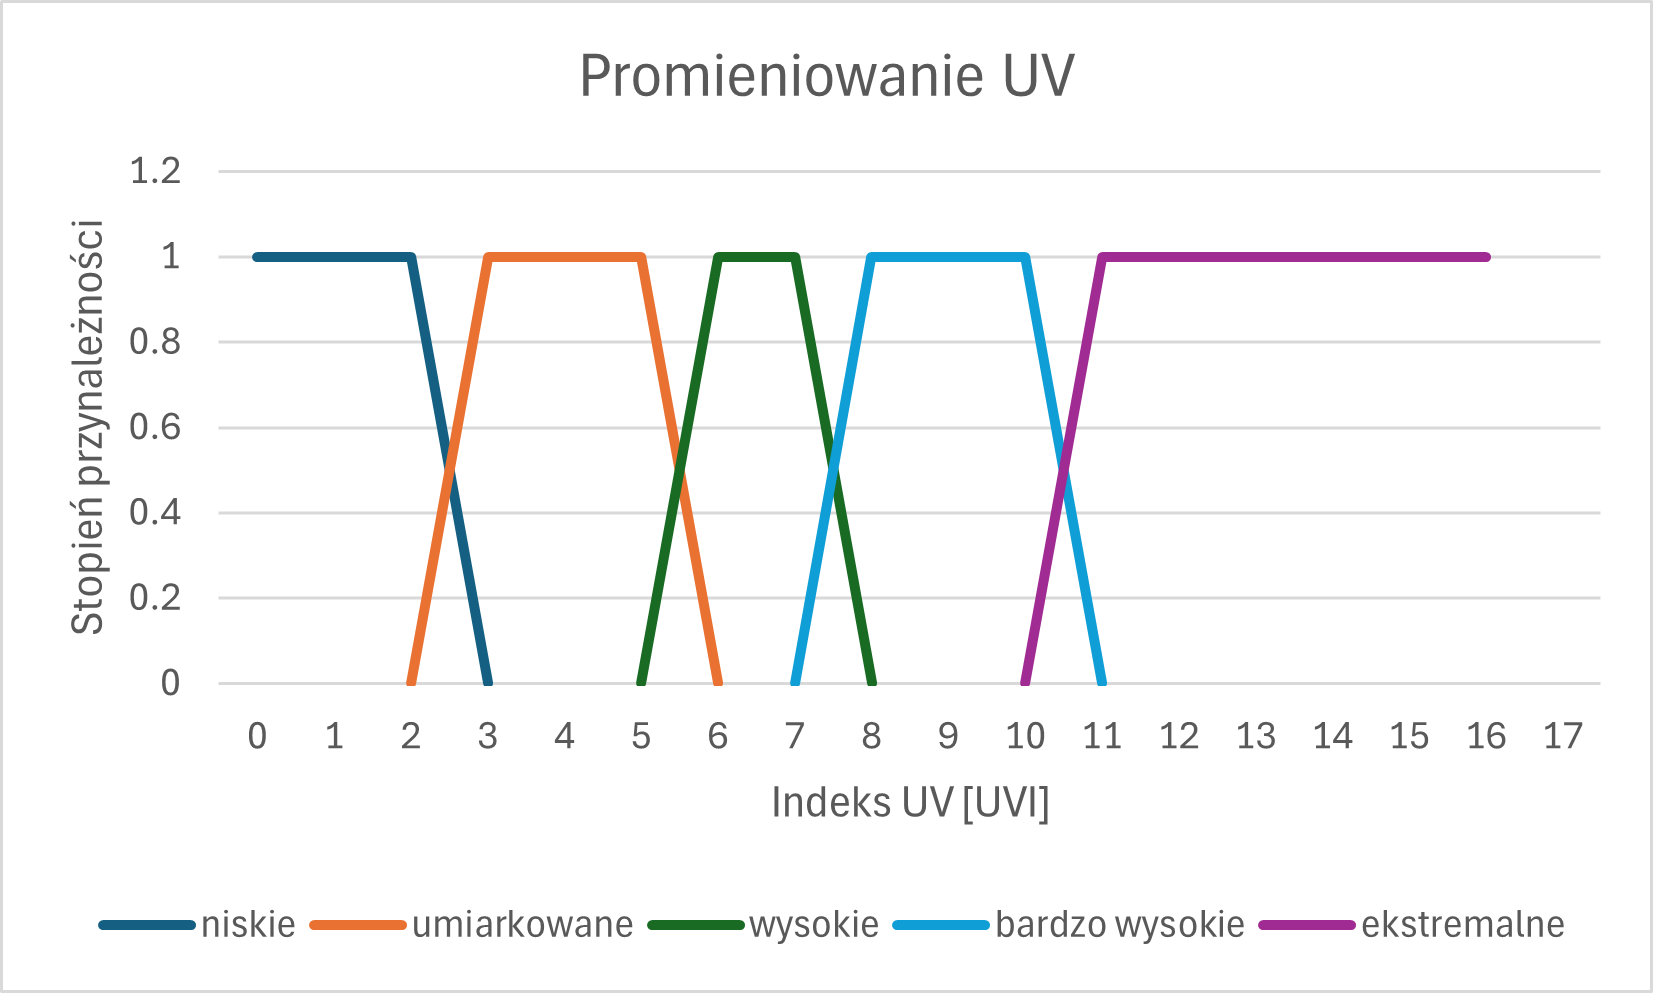
\includegraphics[width=\textwidth]{img/uv.png}
    \caption{Wykres funkcji przynależności dla promieniowania UV.}
    \end{figure}

    \item air\_quality\_Carbon\_Monoxide
            \begin{equation}
            L_8 = \langle \mathcal{L}_8, H_8, \mathcal{X}_8 \rangle
        \end{equation}
        gdzie: $\mathcal{L}_8$ – zanieczyszczenie CO2, $H_8$ – \{normalne, niezdrowe, niebezpieczne\}, $\mathcal{X}_8 = [0, 2220]$. \\
        Poniżej wzory dla wszystkich możliwych etykiet.

\begin{equation}
\mu_{\text{normalne}}(x) =
\begin{cases}
1, & x \in [0, 200] \\
\frac{400 - x}{200}, & x \in (200, 400] \\
0, & \text{w przeciwnym razie}
\end{cases}
\end{equation}

\begin{equation}
\mu_{\text{niezdrowe}}(x) =
\begin{cases}
\frac{x - 200}{200}, & x \in (200, 400] \\
1, & x \in (400, 800] \\
\frac{1000 - x}{200}, & x \in (800, 1000) \\
0, & \text{w przeciwnym razie}
\end{cases}
\end{equation}

\begin{equation}
\mu_{\text{niebezpieczne}}(x) =
\begin{cases}
\frac{x - 800}{200}, & x \in (800, 1000] \\
1, & x > \ in (1000, 2220] \\
0, & \text{w przeciwnym razie}
\end{cases}
\end{equation}

    \begin{figure}[H]
    \centering
    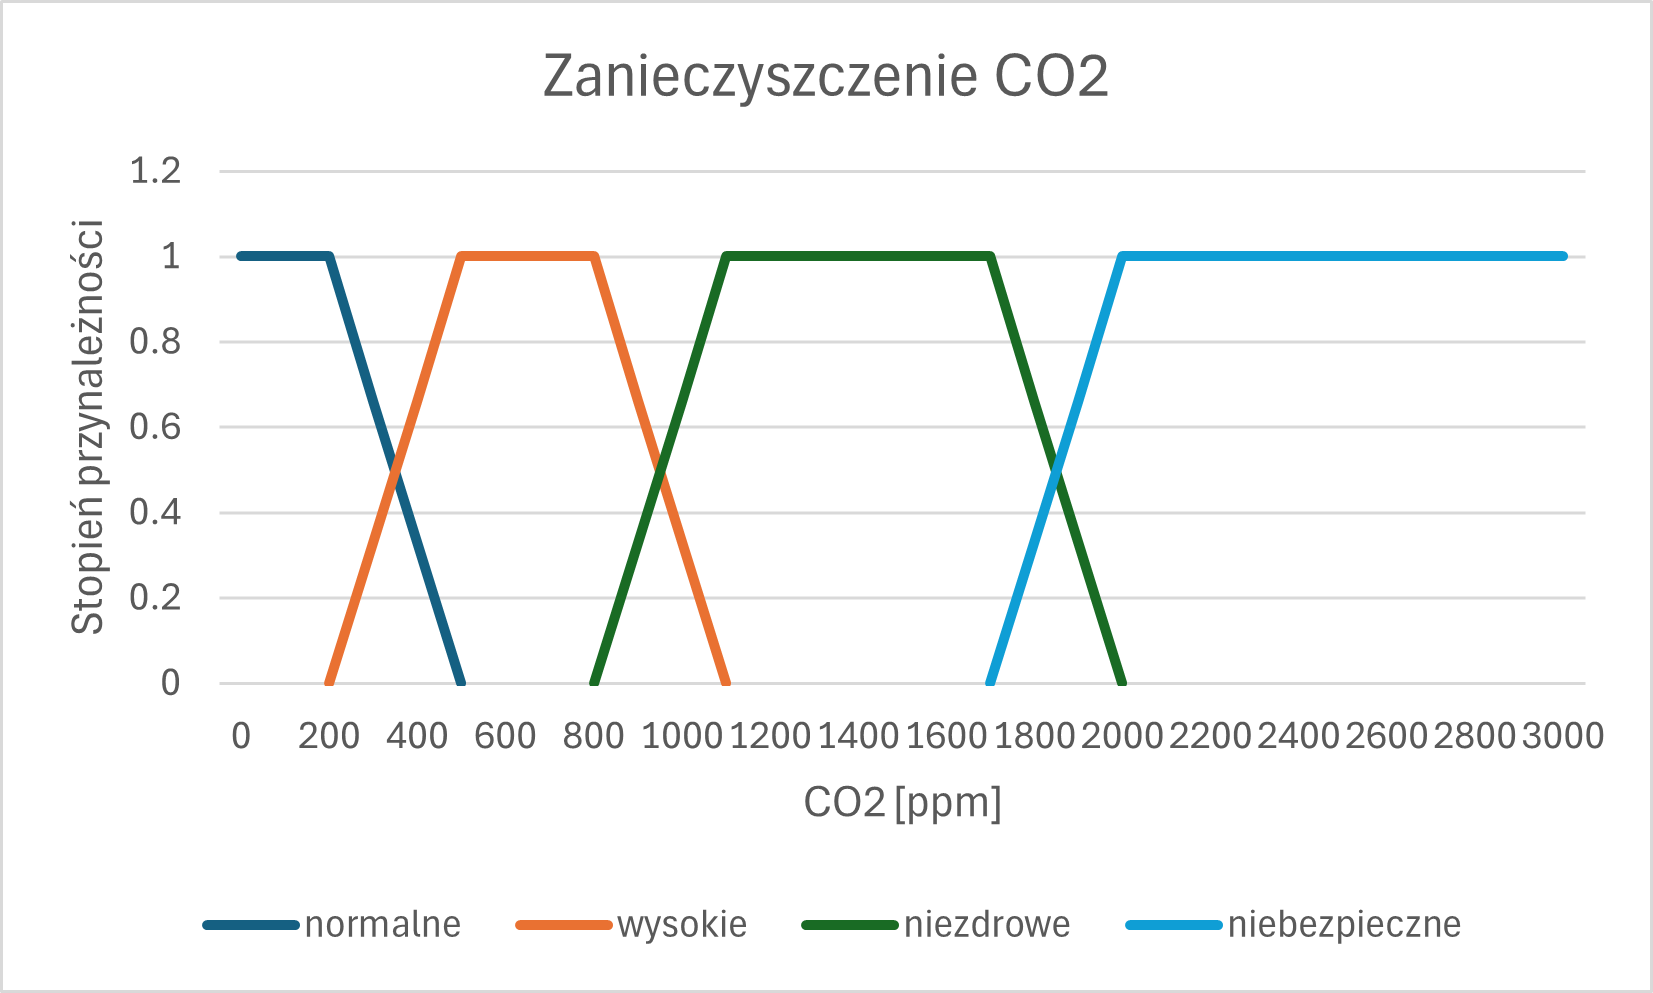
\includegraphics[width=\textwidth]{img/co.png}
    \caption{Wykres funkcji przynależności dla zanieczyszczenia CO2.}
    \end{figure}
    
    \item air\_quality\_Nitrogen\_dioxide
                \begin{equation}
            L_9 = \langle \mathcal{L}_9, H_9, \mathcal{X}_9 \rangle
        \end{equation}
        gdzie: $\mathcal{L}_9$ – zanieczyszczenie NO2, $H_9$ – \{normalne, niezdrowe, niebezpieczne\}, $\mathcal{X}_9 = [0, 428]$. \\
        Poniżej wzory dla wszystkich możliwych etykiet.

\begin{equation}
\mu_{\text{normalne}}(x) =
\begin{cases}
1, & x \in [0, 50] \\
\frac{100 - x}{50}, & x \in (50, 100] \\
0, & \text{w przeciwnym razie}
\end{cases}
\end{equation}

\begin{equation}
\mu_{\text{niezdrowe}}(x) =
\begin{cases}
\frac{x - 100}{50}, & x \in (100, 150] \\
1, & x \in (150, 200] \\
\frac{250 - x}{50}, & x \in (200, 250) \\
0, & \text{w przeciwnym razie}
\end{cases}
\end{equation}

\begin{equation}
\mu_{\text{niebezpieczne}}(x) =
\begin{cases}
\frac{x - 200}{50}, & x \in (200, 250] \\
1, & x \in (250, 428] \\
0, & \text{w przeciwnym razie}
\end{cases}
\end{equation}

        \begin{figure}[H]
    \centering
    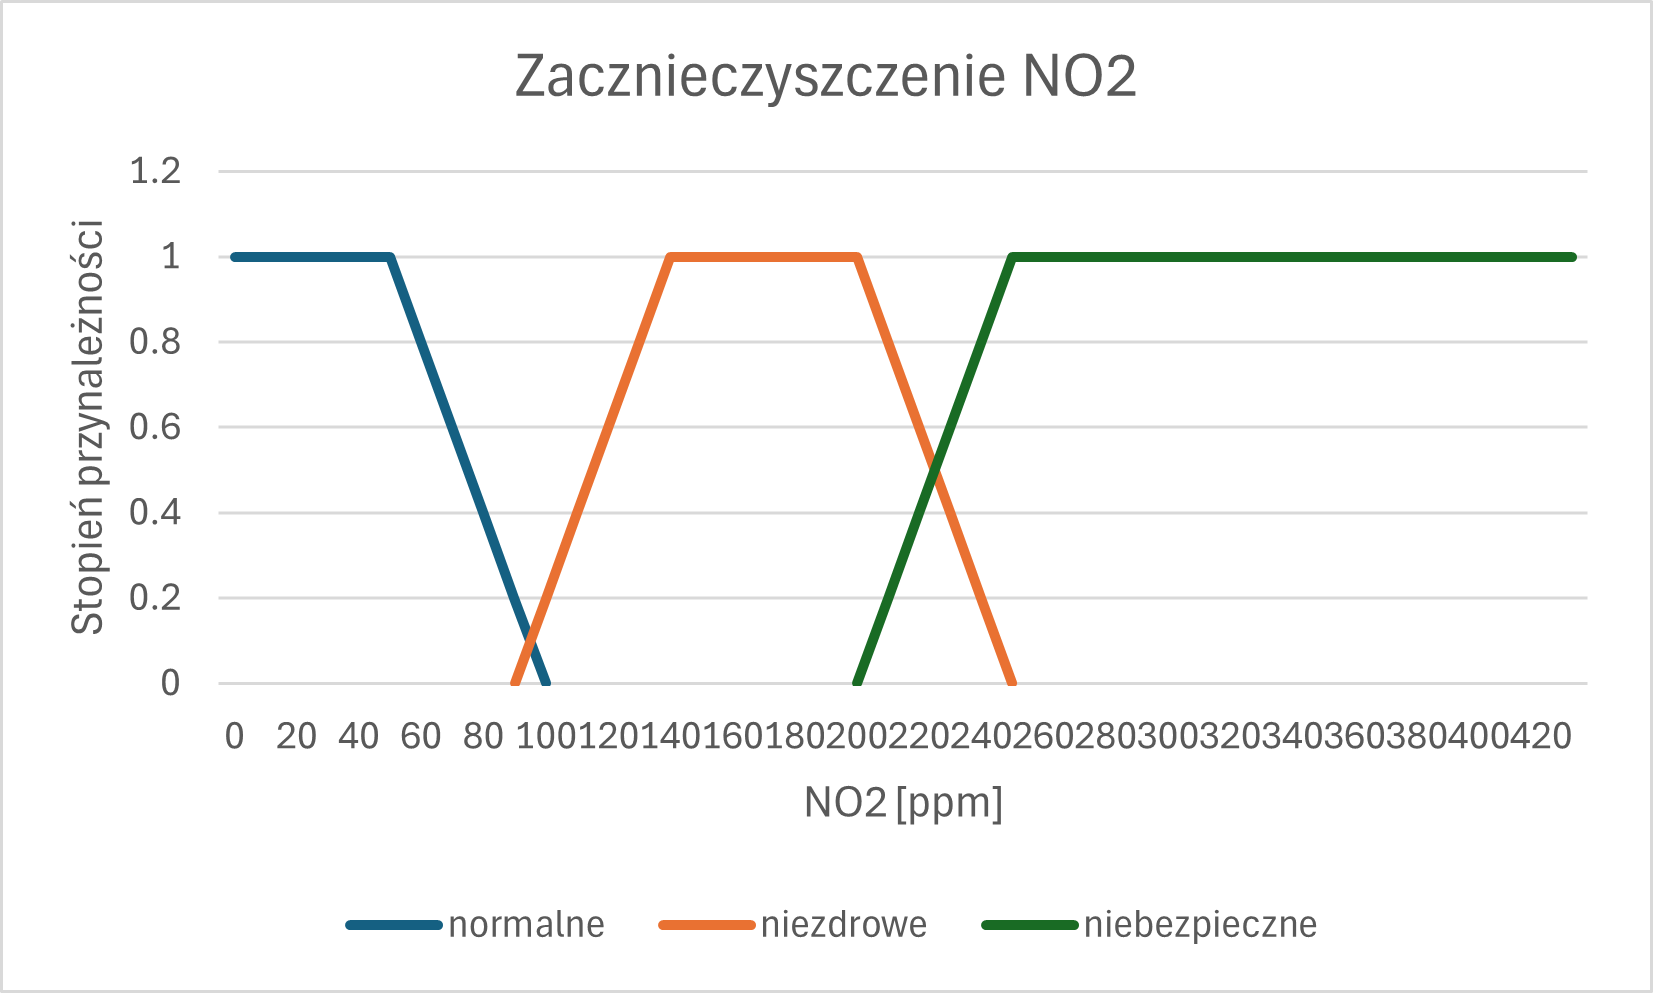
\includegraphics[width=\textwidth]{img/no.png}
    \caption{Wykres funkcji przynależności dla zanieczyszczenia no2.}
    \end{figure}
        
    \item Indeks jakości powietrza
                \begin{equation}
            L_10 = \langle \mathcal{L}_10, H_10, \mathcal{X}_10 \rangle
        \end{equation}
        gdzie: $\mathcal{L}_10$ – jakość powietrza, $H_10$ – \{bardzo dobra, dobra, umiarkowana, zła, bardzo zła\}, $\mathcal{X}_10 = [1, 10]$. \\
        Poniżej wzory dla wszystkich możliwych etykiet.

\begin{equation}
\mu_{\text{bardzo\_dobra}}(x) =
\begin{cases}
1, & x \in [1, 2] \\
\frac{3 - x}{1}, & x \in (2, 3] \\
0, & \text{w przeciwnym razie}
\end{cases}
\end{equation}

\begin{equation}
\mu_{\text{dobra}}(x) =
\begin{cases}
\frac{x - 2}{1}, & x \in (2, 3] \\
1, & x \in (3, 4] \\
\frac{5 - x}{1}, & x \in (4, 5) \\
0, & \text{w przeciwnym razie}
\end{cases}
\end{equation}

\begin{equation}
\mu_{\text{umiarkowana}}(x) =
\begin{cases}
\frac{x - 4}{1}, & x \in (4, 5] \\
1, & x \in (5, 6] \\
\frac{7 - x}{1}, & x \in (6, 7) \\
0, & \text{w przeciwnym razie}
\end{cases}
\end{equation}  

                \begin{equation}
                    \mu_{\text{zła}}(x) =
                    \begin{cases}
                    \frac{x - 6}{1}, & x \in (6, 7] \\
                    1, & x \in (7, 8] \\
                    \frac{9 - x}{1}, & x \in (8, 9)\\
                    0, & \text{w przeciwnym razie} \\
                    \end{cases}
                \end{equation}

                \begin{equation}
                    \mu_{\text{bardzo zła}}(x) =
                    \begin{cases}
                    \frac{x - 8}{1}, &  x \in (8, 9] \\
                    1, & x \in (9, 10] \\
                    0, & \text{w przeciwnym razie} \\
                    \end{cases}
                \end{equation}

            \begin{figure}[H]
    \centering
    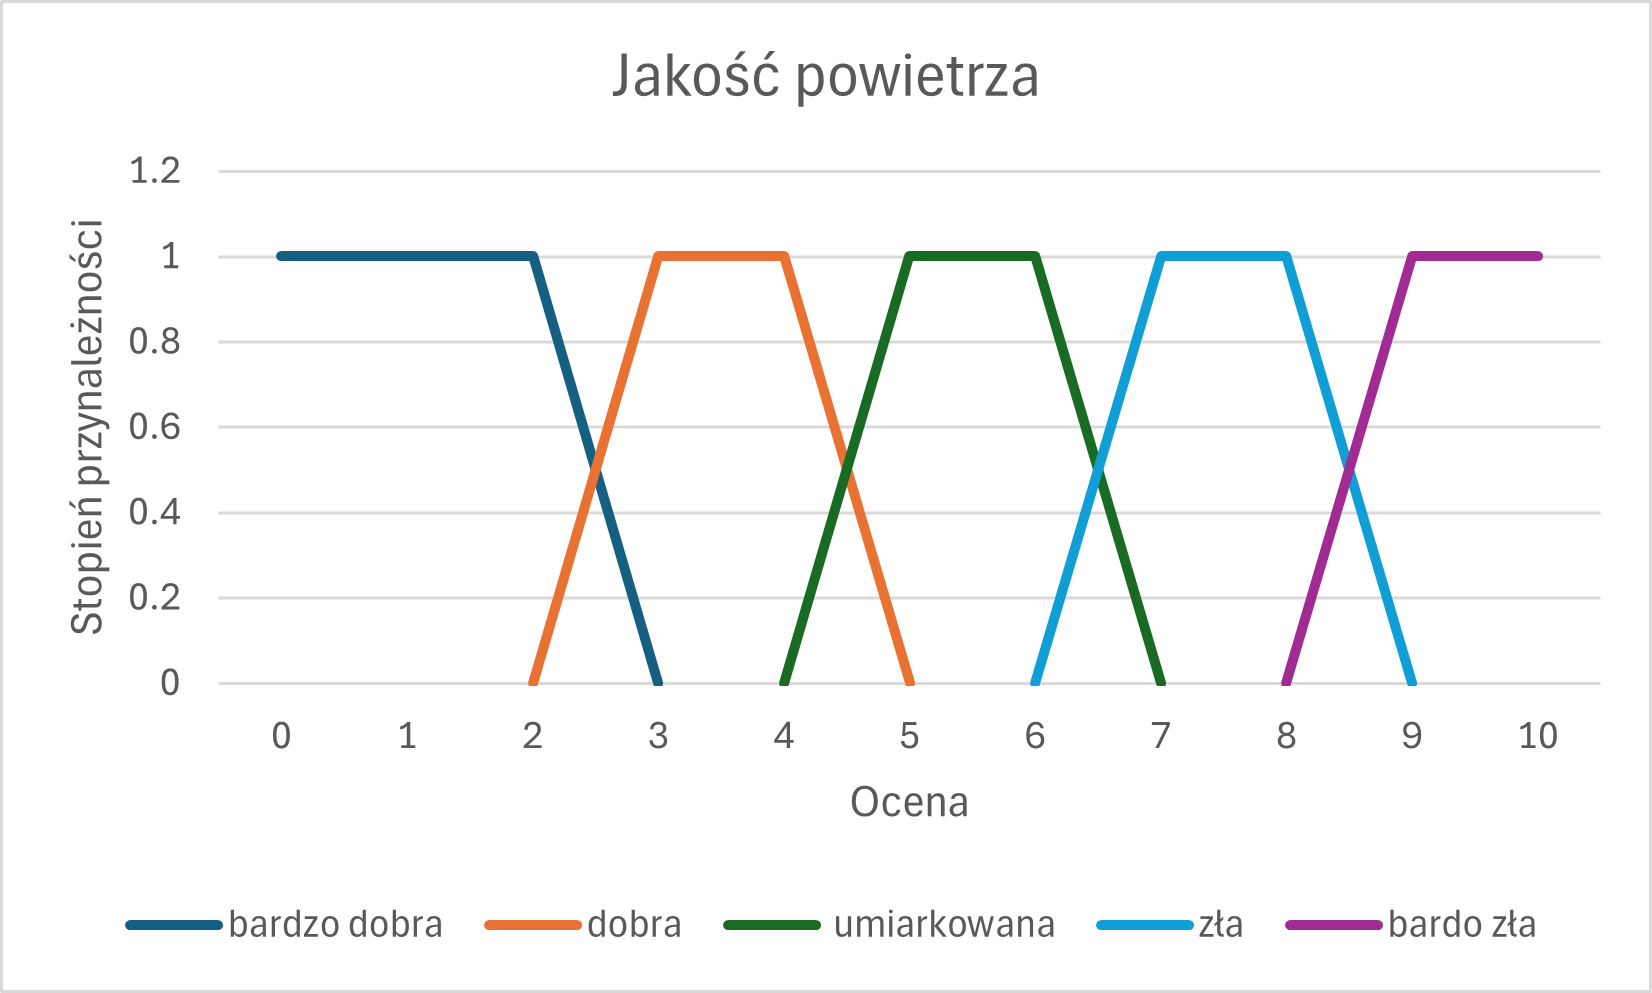
\includegraphics[width=\textwidth]{img/air.png}
    \caption{Wykres funkcji przynależności dla jakości powietrza.}
    \end{figure}
\end{enumerate}


Zmienne lingwistyczne dla wybranych 10 atrybutów z bazy danych, przedstawione w
formie wykresów funkcji przynależności i wzorów analitycznych, wymienione etykiety oraz objaśnione wszystkie
symbole ułatwiające czytelnikowi ich zrozumienie \cite{zadrozny06}. {\bf Zbędne jest
cytowanie definicji}. Konieczne {\bf precyzyjnie podane przestrzenie rozważań każdej
zmiennej lingwistycznej}, wzory i wykresy dla każdej wartości/etykiety.
Nadmiarowe rysunki i wzory mogą być podane w załącznikach. 

\subsection{Kwantyfikatory lingwistyczne (liczności obiektów)}
Poniżej zostały zaprezentowane kwantyfikatory lingwistyczne wraz z ich wzorami analitycznymi oraz wykresem funkcji przynależności.
\begin{itemize}
    \item wcale
        \begin{equation}
            \mu_{\text{wcale}}(x) =
        \begin{cases}
        \dfrac{0.2 - x}{0.2 - 0}, & 0 < x < 0.2 \\
        0, & \text{w przeciwnym razie}
        \end{cases}
        \end{equation}
    \item trochę
        \begin{equation}
            \mu_{\text{trochę}}(x) =
\begin{cases}
\dfrac{0.3 - x}{0.3 - 0.1}, & 0.15 < x < 0.45 \\
0, & \text{w przeciwnym razie}
\end{cases}
        \end{equation}
    \item około połowa
        \begin{equation}
\mu_{\text{około połowa}}(x) =
\begin{cases}
\dfrac{x - 0.3}{0.5 - 0.3}, & 0.35 < x \leq 0.5 \\
\dfrac{0.7 - x}{0.7 - 0.5}, & 0.5 < x < 0.75 \\
0, & \text{w przeciwnym razie}
\end{cases}
        \end{equation}
    \item{wiele}
        \begin{equation}
            \mu_{\text{wiele}}(x) =
\begin{cases}
\dfrac{x - 0.4}{0.6 - 0.4}, & 0.55 < x \leq 0.75 \\
\dfrac{0.8 - x}{0.8 - 0.6}, & 0.75 < x < 0.9 \\
0, & \text{w przeciwnym razie}
\end{cases}
        \end{equation}
    \item{prawie wszystkie}
        \begin{equation}
            \mu_{\text{prawie wszystkie}}(x) =
\begin{cases}
\dfrac{x - 0.7}{0.9 - 0.7}, & 0.7 < x \leq 0.9 \\
\dfrac{1 - x}{1 - 0.9}, & 0.9 < x < 1 \\
0, & \text{w przeciwnym razie}
\end{cases}
        \end{equation}
\end{itemize}

        \begin{figure}[H]
    \centering
    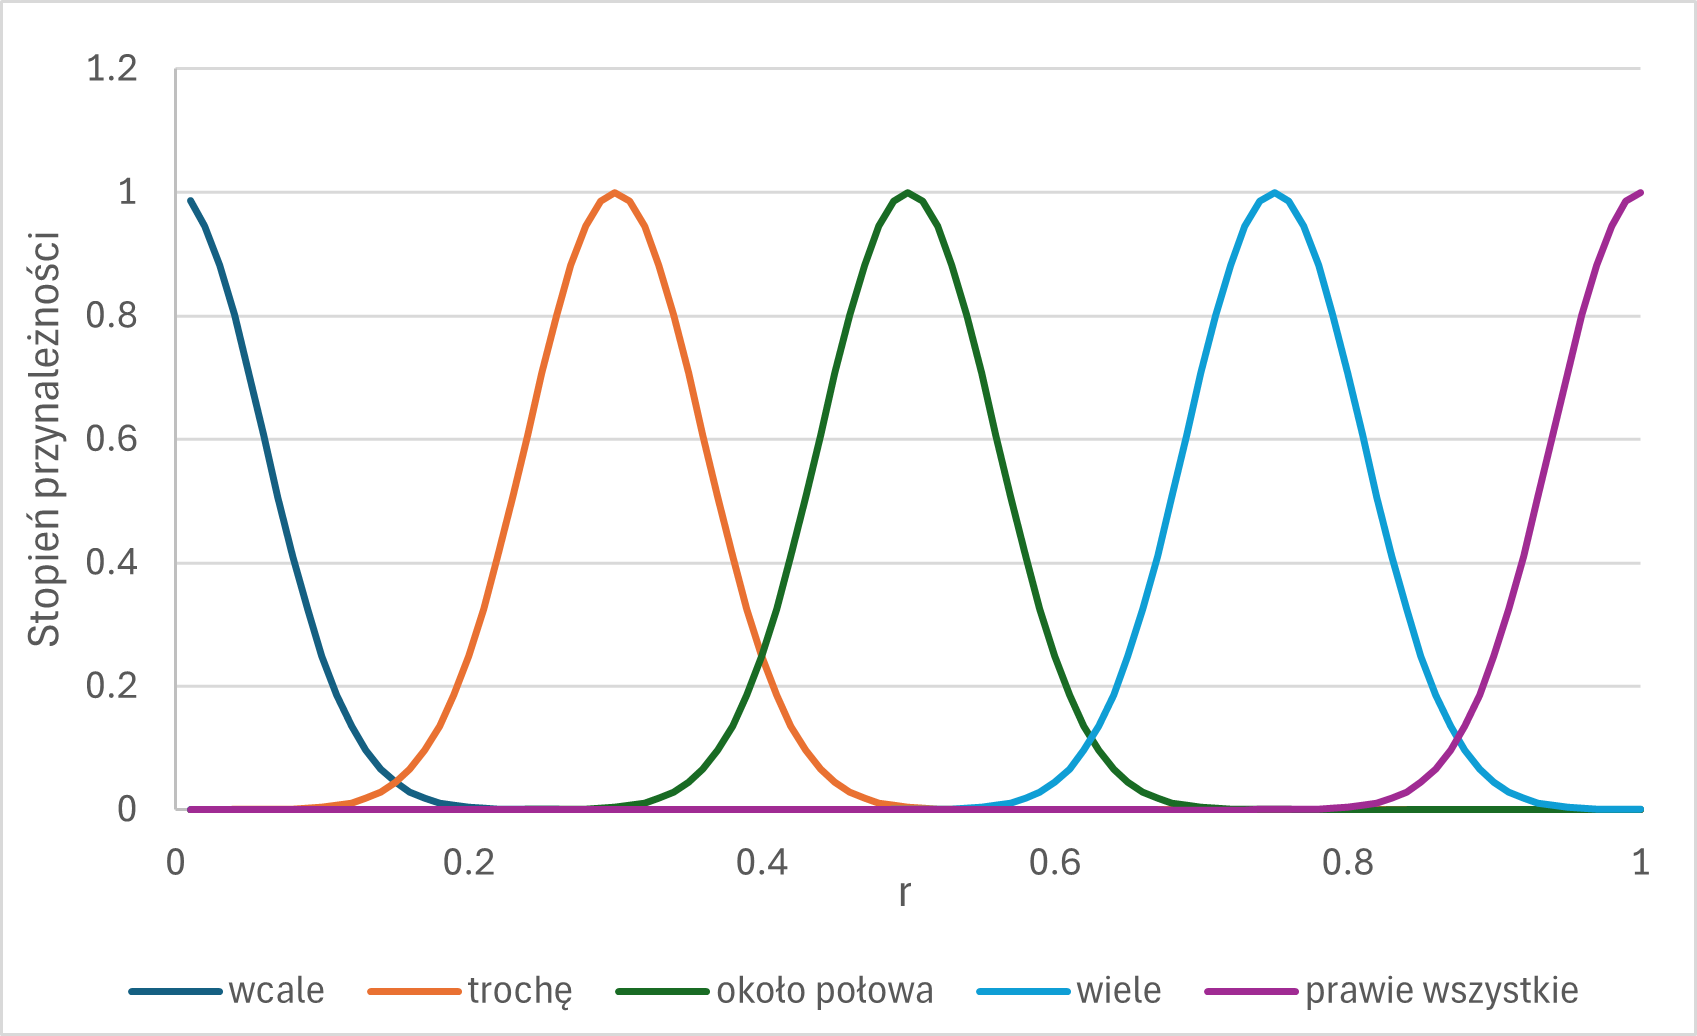
\includegraphics[width=\textwidth]{img/a.png}
    \caption{Funkcja przynależności dla wybranych kwantyfikatorów lingwistycznych.}
    \end{figure}


Jw. kwantyfikatory lingwistyczne -- opisane etykietami, wykresami funkcji
przynależności i wzorami analitycznymi. Uzasadnione wiedzą dziedzinową  
{\bf zakresy i etykiety}. Precyzyjnie podane przestrzenie rozważań każdego kwantyfikatora 
lingwistycznego/rozmytego, wzory i wykresy dla każdej wartości/etykiety. Opisy własne z~przypisami do literatury, tak by inżynier innej specjalności zrozumiał dalszy
opis tego konkretnego ćwiczenia/eksperymentu. 
Nadmiarowe rysunki i wzory mogą być podane w załącznikach.  

\section{Narzędzia obliczeniowe: wybór/implementacja. Diagram UML klas do obliczeń rozmytych i generowania podsumowań}
\noindent {\bf Sekcja uzupełniona jako efekt zadania Tydzień 10 wg Harmonogramu Zajęć na WIKAMP KSR.}

Diagram UML i zwięzły opis pakietu obliczeń rozmytych: źródło pakietu
(zewnętrzny/własny/hybrydowy), przypis do literatury/źródeł. Krótka charakterystyka
najważniejszych klas i podstawowych dla zadania ich metod. \\

Wersja JRE i inne wymogi niezbędne do uruchomienia aplikacji przez użytkownika na własnym komputerze. 

\section{ Jednopodmiotowe podsumowania lingwistyczne. Miary jakości, podsumowanie optymalne}
Wyniki kolejnych eksperymentów wg punktów 2.-4. opisu projektu 2.  Listy podsumowań
jednopodmiotowych i tabele/rankingi podsumowań dla danych atrybutów obowiązkowe i dokładnie opisane w ,,captions'' (tytułach), konieczny opis kolumn i wierszy tabel. Dla każdego podsumowania podane miary jakości oraz miara jakości podsumowania
optymalnego. {\bf Wzorów podsumowań ani miar nie należy przepisywać ani cytować, wystarczy podać literaturę, ale
należy skomentować co oznaczają i jaką informacje niosą wybrane miary w wybranych
przypadkach.}\\
\noindent {\bf Sekcja uzupełniona jako efekt zadania Tydzień 11 wg Harmonogramu Zajęć na WIKAMP KSR.}

\section{Wielopodmiotowe podsumowania lingwistyczne i~ich miary jakości} 
Wyniki kolejnych eksperymentów wg punktów 2.-4. opisu projektu 2. Uzasadnienie i
metoda podziału zbioru danych na rozłączne podmioty. Listy podsumowań
wielopodmiotowych i tabele/rankingi podsumowań dla danych atrybutów obowiązkowe i
dokładnie opisane w ,,captions'' (tytułach), konieczny opis kolumn i wierszy tabel.
{\bf Wzorów podsumowań ani miar nie należy przepisywać ani cytować, wystarczy podać literaturę, ale
należy skomentować co oznaczają i jaką informacje niosą wybrane miary w wybranych
przypadkach.} Konieczne uwzględnienie wszystkich 4-ch form podsumowań wielopodmiotowych. 
\\ 

** Możliwe sformułowanie zagadnienia wielopodmiotowego podsumowania optymalnego **.\\
\indent {** Ewentualne wyniki realizacji punktu ,,na ocenę 5.0'' wg opisu Projektu 2. i ich porównanie do wyników z
części obowiązkowej **.}\\

\noindent {\bf Sekcja uzupełniona jako efekt zadania Tydzień 12 wg Harmonogramu Zajęć
na WIKAMP KSR.}


\section{Dyskusja, wnioski}
Dokładne interpretacje uzyskanych wyników w zależności od parametrów klasyfikacji
opisanych w punktach 3.-4 opisu Projektu 2. 
Omówić i wyjaśnić napotkane problemy (jeśli były). Każdy wniosek/problem powinien mieć poparcie
w przeprowadzonych eksperymentach (odwołania do konkretnych wyników: tabel i miar
jakości). Ocena które podsumowania i dlaczego niosą najistotniejsze informacje
i które ich miary jakości mają małe albo duże znaczenie dla wiarygodności i jakości otrzymanych
agregacji/podsumowań.  \\
\underline{Dla końcowej oceny jest to najważniejsza sekcja} sprawozdania, gdyż prezentuje poziom
zrozumienia rozwiązywanego problemu.\\

** Możliwości kontynuacji prac w obszarze logiki rozmytej i wnioskowania rozmytego, zwłaszcza w kontekście pracy inżynierskiej,
magisterskiej, naukowej, itp. **\\

\noindent {\bf Sekcja uzupełniona jako efekt zadań Tydzień 11 i Tydzień 12 wg
Harmonogramu Zajęć na WIKAMP KSR.}


\section{Braki w realizacji projektu 2.}
Wymienić wg opisu Projektu 2. wszystkie niezrealizowane obowiązkowe elementy projektu, ewentualnie
podać merytoryczne (ale nie czasowe) przyczyny tych braków. 


\begin{thebibliography}{99}
\bibitem{baza} World Weather Repository - kaggle, \url{https://www.kaggle.com/datasets/nelgiriyewithana/global-weather-repository?resource=download}. [dostęp 18.05.2025r.]
 \bibitem{niewiadomski19} A. Niewiadomski, Zbiory rozmyte typu 2. Zastosowania w reprezentowaniu informacji.  Seria „Problemy współczesnej informatyki” pod redakcją L. Rutkowskiego. Akademicka Oficyna Wydawnicza EXIT, Warszawa, 2019.
\bibitem{zadrozny06} S. Zadrożny, Zapytania nieprecyzyjne i lingwistyczne podsumowania baz danych, EXIT, 2006, Warszawa
\bibitem{niewiadomski08} A. Niewiadomski, Methods for the Linguistic Summarization of Data: Applications of Fuzzy Sets and Their Extensions, Akademicka Oficyna Wydawnicza EXIT, Warszawa, 2008.
\end{thebibliography}

Literatura zawiera wyłącznie źródła recenzowane i/lub o potwierdzonej wiarygodności,
możliwe do weryfikacji i cytowane w sprawozdaniu. 
\end{document}
